\documentclass[../main.tex]{subfiles}
\makeatletter
\@ifundefined{fromRoot}{%
  \newcommand{\fromRoot}[1]{../#1}
  
  \usepackage{xr}
  \externaldocument{../main}
}{}

\def\input@path{{\subfix{../}}}
%or: \def\input@path{{/path/to/folder/}{/path/to/other/folder/}}
\makeatother

\graphicspath{{\subfix{../}}}

\hypersetup{
    pdfauthor   = {Mael Tourres},
    pdftitle    = {Th\`{e}se (Chapitre 3)},
    pdfsubject  = {Th\`{e}se (Chapitre 3)},
%    pdfkeywords = {mots-cl\'{e}s},
}

\begin{document}
\selectlanguage{french}
%
%
%
%méthodologie + SISD
\chapter{Méthodologie de conception et d'implantation d'extensions} 
\label{chapter:3}
\chaptermark{Jeux d'instructions à 2 registres}
%
% 
%
%
%

Ce chapitre vise à d'introduire les travaux effectués afin de proposer des jeux d'instruction spécialisés dédiés au décodage de codes correcteurs d'erreurs (CCE). 

Dans un premier temps, le flot d'analyse et d'exploration mis en œuvre est introduit, ainsi que les contraintes architecturales retenues. L'objectif est la mise en place d'une approche permettant d'extraire les instructions ou blocs d'instructions qui affectent les performances des décodeurs de CCE en termes de temps d'exécution sur des cibles de type cœur de processeur. 

À titre d'exemple, il est ensuite présenté quelques sous-parties des codes logiciels pour décodeurs les plus performants (en termes de débit) de l'état de l'art, pour les différentes familles de codes correcteurs, afin d'illustrer certains des motifs d'instructions sélectionnés. 

La pertinence du flot d'exploration et les nouvelles instructions opérant sur des données scalaires sont ensuite validées par des expérimentations sur des circuits FPGA. Ces dernières sont réalisées grâce à l'enrichissement de cœurs de processeurs \textit{open-source} de type RISC-V. 
L'analyse des résultats obtenus permet d'évaluer l'apport des extensions proposées sur le temps d'exécution des algorithmes de décodage considérés, mais également leurs impacts sur l'augmentation de la complexité matérielle. 



\etocsetnexttocdepth{4}
\etocsettocstyle{{\large \hspace{-1.5 em} \textbf{} \hfill}\vspace{-2.5 em}\\\par\noindent\rule{\linewidth}{1 pt}\vspace{-.2 em}}{\par\noindent\rule{\linewidth}{1 pt}\\}
\localtableofcontents
%
%
%
%
%
\section{Introduction}
%
%
%
%
%
%
Cette première partie du chapitre a pour but de présenter le flot de conception utilisé dans le cadre de cette thèse. 
En ce sens, est introduit, pour chacun des algorithmes de décodeur de CCE considérés dans cette étude, les instructions ou séquences d'instructions ayant des impacts négatifs sur leurs performances générales. 
La sélection des codes logiciels C/C++ retenus, est effectuée sur la base de leur capacité à être implantés efficacement sur des cibles de type processeur généralistes. 
Les algorithmes retenus constituent, à ce jour, l'état de l'art pour les cibles considérées et leurs performances ont été validées par des simulations BER/FER. 

L'objectif est de déterminer, au cœur des algorithmes de décodage, les instructions ou groupes d'instructions récurrents les moins efficaces/pertinentes sur architectures programmables et qui puissent avoir une implantation matérielle \textit{simple}.
La sélection de ces motifs d'instructions est basée sur les critères suivants:  
\begin{itemize}
    \item les instructions sélectionnées doivent être compatibles avec la plupart des jeux d'instructions standards ; \textit{i.e.} deux registres d'entrée \textit{\textbf{S}}ource \textit{rS1 et rS2} et un registre de sortie \textit{\textbf{D}}estination \textit{rD};
    \item les nouvelles instructions doivent pouvoir s'exécuter sur un seul cycle d'horloge, sans provoquer de rupture de pipeline ;
    \item lorsque possible, les données internes sont codées 8 bits signés.
\end{itemize}
Ce dernier point est retenu, car il présente le meilleur compromis entre complexité d'implantation, indépendamment de la cible, et les performances de décodage. 

Pour mettre en œuvre cette approche, un flot de conception a été mis au point et schématisé dans la figure \ref{flot}. 
Il est important de rappeler que les codes logiciels décrivant le processus de décodage des CCE ont été optimisés afin d'exposer les séquences d'instructions qui peuvent être réduites à une seule.


%
%
%
%
\section{Descriptif du flot de conception} 
%
%
%
%

Dans un premier temps (\textit{cf.} figure \ref{flot}), les différents codes logiciels (\textit{a.k.a. kernels (\ding{182}} dans la figure) sont exécutés sur les cibles sélectionnées (\ding{188}).
Pour toutes les familles de CCE étudiées, nous sommes partis des meilleurs algorithmes de l'état de l'art, re-codés pour un contexte embarqué. Cette première étape permet d'extraire les instructions les plus onéreuses en temps d'exécution et qui répondent aux critères définis précédemment (\ding{183}). Cela a permis d'établir pour chaque famille de CCE une liste d'instructions à intégrer (\ding{184}).

%%%%%%%%%%%%%%%%%%%%%%%%%%%%%%%%%
\begin{figure}
\centering
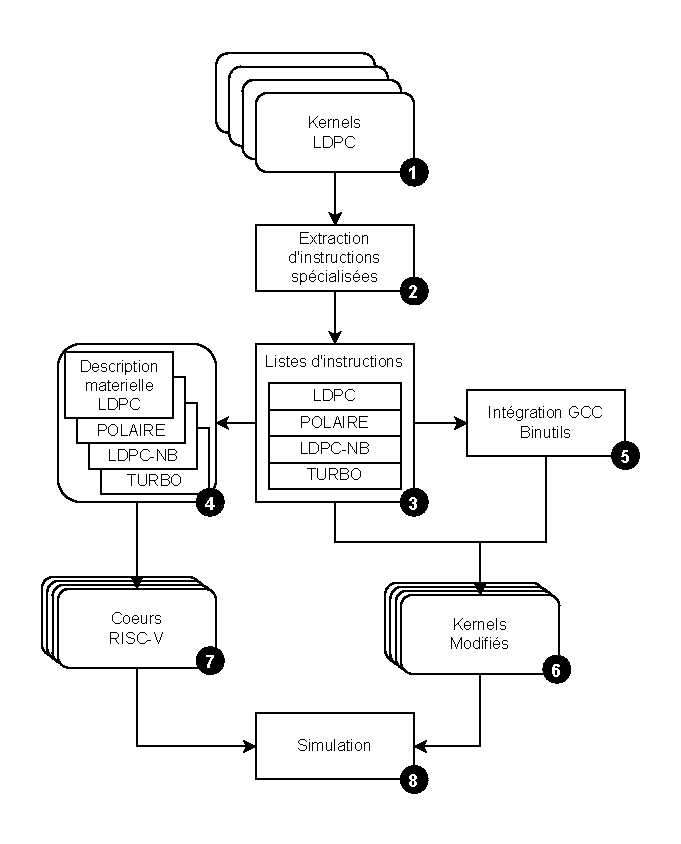
\includegraphics[scale=1]{chapter3/figs/flot.pdf}
\caption{ Flot de conception global intégrant l'analyse et la sélection des instructions, l'intégration dans le flot de compilation et la mesure des performances.}
\label{flot}
\end{figure}
%%%%%%%%%%%%%%%%%%%%%%%%%%%%%

L'ensemble de ces instructions ont, par la suite, été décrites au niveau RTL en \textit{Verilog} ou \textit{System-Verilog} (\ding{185}). Ensuite, leur ajout dans l'ISA des cœurs RISC-V (\ding{188}) \cite{ArchiRISC:V} à été effectué.
Naturellement, afin que les kernels décrits en langage C/C++ puissent exploiter ces nouvelles instructions (\ding{184}), il a été nécessaire de les adapter en remplaçant les sections de codes initiales par des invocations en assembleur à ces nouvelles fonctionnalités (\ding{187}).
Il a été également primordial de les intégrer dans les chaînes de compilation des cœurs ciblés via GCC/Binutils (\ding{186}) pour permettre la génération de programmes exécutables.
Enfin, une dernière étape (\ding{189}) a permis de valider les performances des kernels modifiés sur ces cœurs étendus, grâce à des tests réalisés en simulation ou par prototypage sur des circuits FPGA (Digilent Nexys 4 et Digilent Genesys 2).
Ce sont donc ces versions incluant notre kit d'instructions qui sont alors utilisées pour les études expérimentales présentées dans ce chapitre.

%%%%%%%%%%%%%%%%%%%%%%%%%%%%%
\begin{figure}
\centering
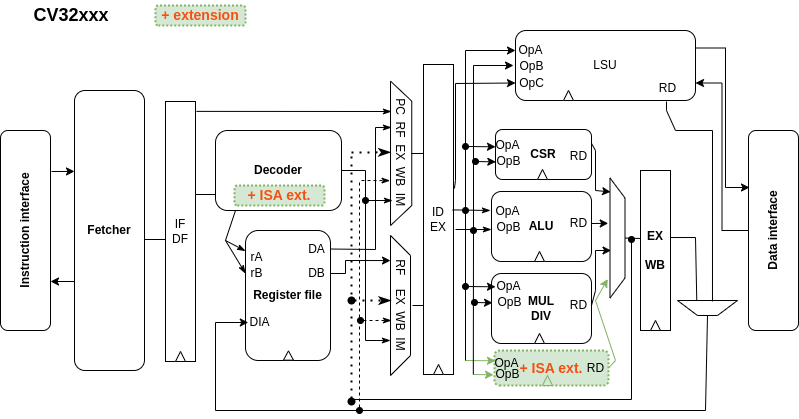
\includegraphics[scale=0.5]{chapter3/figs/CV32xxx+Ext.png}
\caption{Principe d'insertion d'instruction spécialisées dans un cœur RISC-V (schéma pédagogique du cœur \cite{ArchiRISC:V})}
\label{RV2regs}
\end{figure}
%%%%%%%%%%%%%%%%%%%%%%%%%%%%%

La figure \ref{RV2regs} montre, sur l'exemple d’un cœur de processeur à l'architecture simplifiée, mais proche d'un RISC-V CV32 \cite{ArchiRISC:V}, les principales parties concernées par l'ajout de nos extensions d'instructions.
Ces nouvelles instructions proposées sont encodées selon le format de type R présenté dans \ref{R_instruction}, qui permet un mécanisme d'échange de données registres vers registres, relativement simple et direct. Ce type d'encodage mémorise l'\textit{OpCode} sur les 7 bits de poids faibles du registre d'instruction. Les adresses de registres sont passées dans les champs \textit{rS1,rS2} pour les sources et \textit{rD} pour la destination. Les champs \textit{funct7} et \textit{funct3} sont utilisés pour identifier l'instruction.

%%%%%%%%%%%%%%%%%%%%%%%%%%%%%
\begin{table}[]
    \centering
    \begin{tabular}{l|l}
         \textbf{Champ} & \textbf{Bits}  \\
         \bottomrule
         Opcode                 & [6:0]  \\
         Registre destination   & [11:7]  \\
         Fonction 3             & [14:12]  \\
         Registre source 1      & [19:15]  \\
         Registre source 2      & [24:20]  \\
         Fonction 7             & [31:25]  \\
    \end{tabular}
    \caption{Format 32 bits standardisé pour les instructions de type R (2 registres d'entrées) dans la spécification RISC-V.}
    \label{R_instruction}
\end{table}
%%%%%%%%%%%%%%%%%%%%%%%%%%%%%

Bien que d'autres formats d'instructions existent dans la spécification RISC-V, le format de type R est suffisant pour enrichir le jeu d'instructions. 

On constate ainsi qu'après l'étape de \textit{Fetch} de l'instruction, l'étape de \textit{Decoder} doit être mise à jour pour reconnaître les nouvelles instructions et ainsi générer des signaux de contrôle adaptés. 
De même, une unité de calcul spécifique à notre kit d'instructions doit être ajoutée dans l'architecture du système.
Le reste de l'architecture du processeur n'est pas affecté par l'insertion de ces nouvelles instructions.    
Les expérimentations montrent les gains en performances que ces modifications peuvent apporter pour différents cœurs de processeur RISC-V et pour différents codes correcteurs, en fonction du parallélisme qui sera utilisé.
Toutefois, ce type d’architecture avec 2 registres d’entrée et 1 registre de sortie se révèle peu efficace pour certains CCE, comme cela sera démontré par la suite. 

La suite de ce chapitre présente, pour chacune des familles de CCE, les motifs d'instructions qui ont été sélectionnés.

%
%
%
%
\subsection{Amélioration du décodage logiciel des codes LDPC}
%
%
%
%
Depuis leur redécouverte, il y a une trentaine d'années, les codes LDPC ont vu la mise au point de nombreux algorithmes de décodage qui offrent à la fois de bonnes propriétés d'implantation et un pouvoir élevé en termes de correction d'erreurs. Ces derniers ont donné lieu à une multitude d'architectures matérielles tant sur cible ASIC \cite{LDPC:APPROX:3} que FPGA \cite{LDPC:APPROX:4}. 

Dans le cadre de ces travaux de thèse, l'algorithme considéré est le \textit{\textbf{M}in-\textbf{S}um/\textbf{O}ffset \textbf{M}in-\textbf{S}um} (\textit{MS/OMS}) offrant le meilleur compromis entre complexité d'intégration \textit{vs} et performances de décodage. De manière analogue aux architectures matérielles \cite{LDPC:APPROX:3,LDPC:APPROX:4} et aux implantations logicielles sur cibles multicœurs \cite{BLG:REVUE:TPDS}, la formulation par couche horizontale des calculs de parité a été sélectionnée afin d'accélérer la vitesse de convergence du décodeur. 
L'algorithme de décodage est composé de plusieurs boucles imbriquées permettant le calcul de la parité des nœuds $\bm{C_n}$ et la mise à jour des nœuds de données $\bm{V_n}$. 
Pour ce faire, à chaque \textit{itération} de décodage, l'algorithme va, pour chaque $\bm{C_n}$, actualiser sa valeur de parité à partir des $DegCn$ nœuds de variable qui lui sont connectés. 
À la suite de l'évaluation de sa parité, il va rediffuser des messages à ces mêmes $\bm{V_n}$. Par souci de clarté, un extrait de la formulation de cet algorithme de décodage est présenté ci-après dans le listing \ref{ldpc_code_origin}. Il s'agit d'un code en langage C présentant le calcul de la valeur interne des nœuds de parité à partir des valeurs des accumulateurs et des messages entrants. Cette description simple permet de mettre en exergue la prédominance des opérations arithmétiques et logiques simples par rapport aux accès mémoires et à l'arithmétique sur les pointeurs.



\begin{figure}[!tb]
\begin{lstlisting}[
      label={ldpc_code_origin},
      caption={Formulation en langage C du calcul de mise à jour des noeuds de parité pour un algorihtme MS/OMS avec un ordonnancement horizontal.},
    frame=single,
    backgroundcolor=\color{white},  
    commentstyle=\color{blue}\bfseries,
    keywordstyle=\color{magenta},
    numberstyle=\tiny\color{gray},
    stringstyle=\color{purple},
    basicstyle=\ttfamily\footnotesize,
    numbers=left,
    stepnumber=1,
    numbersep=5pt,                 
    showstringspaces=false,
    tabsize=1,
    breaklines=true,
    language=C++
]
  for(iterations)  // boucle principale
    for(int i = 0; i < nb_CN; i++)  // boucle Cn
      int8_t min1 = 127, min2 = 127, signe = 0;
      int8_t DegCn = deg_Cns[i] ;
      
      //Parcours des Vn connectées au idx_Cn courant 
      for(int j = 0; j < DegCn; j++) // boucle Vn liés au Cn 
        int8_t contr = accuVN[ posVn[j] ] - c2v[j]; 
        contr        = contr >  127 ?  127 : contr;
        contr        = contr < -127 ? -127 : contr;
        
        signe        = signe ^ (contr < 0);
        int8_t abs   = contr > 0 ? contr : -contr;
      
        if(abs < min1) min1 = abs;
        else if(abs < min2) min2 = abs;
\end{lstlisting}
\end{figure}

En analysant cet exemple pédagogique de l'algorithme \ref{ldpc_code_origin}, il est possible de se faire une idée des séquences et/ou groupes d'instructions arithmétiques et logiques pouvant être optimisées : soit par une concaténation d'opérations élémentaires, soit par un ensemble d'instructions réduisant la complexité des calculs utilisés dans les boucles. 
Par exemple, les calculs décrits dans les lignes \textit{8 à 10} réalisent une soustraction signée sur 8 bits suivi d'une saturation symétrique dans l'intervalle $[127, -127]$.

Dans le meilleur des cas, cette séquence d'instructions sera exécutée en cinq cycles d'horloge sur un processeur possédant des instructions conditionnées, ou plus sur un cœur RISC-V qui réaliserait des branchements conditionnels. Pour réduire drastiquement ce temps d'exécution, une approche consiste à créer, par exemple, une instruction capable de réaliser cette soustraction saturée en un seul cycle d'horloge grâce à des ressources matérielles spécifiques. Cette instruction spécifique pourrait ensuite être utilisée dans une version optimisée du code C original.

Afin d'illustrer le résultat de cette transformation, on peut constater dans le listing \ref{ldpc_code_custom} à la ligne \textit{7}, la présence de cette nouvelle instruction \textit{i8\_sub8\_sat127\_pi8}. Celle-ci remplace les instructions des lignes \textit{7, 8} et \textit{9} de l'algorithme originel (listing \ref{ldpc_code_origin}). Cette évolution ne modifie pas le nombre d'itérations de boucle à réaliser, mais réduit la latence de chaque itération et donc minimise le temps d'exécution global.



\begin{figure}[!tb]
\begin{lstlisting}[
    label={ldpc_code_custom},      
    caption={Exemple pédagogique intégrant les instructions du kit ISA.},
    frame=single,
    backgroundcolor=\color{white},  
    commentstyle=\color{blue}\bfseries,
    keywordstyle=\color{magenta},
    numberstyle=\tiny\color{gray},
    stringstyle=\color{purple},
    basicstyle=\ttfamily\footnotesize,
    morekeywords={int8_t},
    numbers=left,
    stepnumber=1,
    numbersep=5pt,                 
    showstringspaces=false,
    tabsize=1,
    breaklines=true,
    language=C
]
for(iterations)  // boucle principale
  for(int i = 0; i < nb_CN; i++)  // boucle Cn
    int8_t min1 = 127, min2 = 127, signe = 0, temp;
    int8_t DegCn = deg_Cns[i];
      
    //Parcours des Vn associés au Cn courant 
    for( int j = 0; j < DegCn; j++ )  // boucle Vn liés au Cn
        int8_t contr    = i8_sub_sat127_pi8(accuVN[ posVn[j] ] - c2v[j]); 
      
        signe           = signe ^ (contr < 0);
        int8_t abs      = i8_abs_pi8(contr); 
     
        temp            = i8_max_pi8(min1, abs);
        min1            = i8_min_pi8(min2, temp);
        min2            = i8_min_pi8(abs, min1); 
\end{lstlisting}
\end{figure}

Pour permettre l'usage de cette nouvelle instruction, il est nécessaire de l'intégrer dans le flot de compilation associé au processeur et plus particulièrement de la provisionner dans l'outil \textit{binutils} comme cela est indiqué dans la figure \ref{flot}. Ainsi, elle devient partie intégrante de l'ISA supportée par le processeur cible et est à la disposition des utilisateurs.

Dans le but de compléter l'intégration de cette nouvelle fonctionnalité, l'opérateur matériel associé doit être décrit au niveau RTL et inséré dans l'architecture de l'\acrshort{ual} du processeur cible. Afin d'illustrer ce travail, la description RTL en langage Verilog de l'opération de soustraction saturée est donné à titre d'exemple dans le listing \ref{SubSat8b_SV}.
    
\begin{figure}[!tb]
\begin{lstlisting}[
    label={SubSat8b_SV},      
    caption={Description matérielle correspondant à l'instruction \textit{i8\_sub\_sat127\_pi8} écrite en System Verilog.},
    frame=single,
    backgroundcolor=\color{white},  
    commentstyle=\color{blue}\bfseries,
    keywordstyle=\color{magenta},
    numberstyle=\tiny\color{gray},
    stringstyle=\color{purple},
    basicstyle=\ttfamily\footnotesize,
    numbers=left,
    stepnumber=1,
    numbersep=5pt,                 
    showstringspaces=false,
    tabsize=1,
    breaklines=true,
    language=verilog
]
//op_a : opérande a de l'UAL 
//op_b : opérande b de l'UAL
//9 bits permettent de contrôler le possible overflow
logic[8:0]  ldpc_res_minus ; 
assign      ldpc_res_minus = $signed(op_a[7:0])-$signed(op_b[7:0]); 

always_comb begin
 unique case (operator)
     UAL_LDPC_SUB_SAT: begin 
     ldpc_subsat_result  = ($signed(ldpc_res_minus) >  9'sd127)?  9'sd127:
                           ($signed(ldpc_res_minus) < -9'sd127)? -9'sd127:
                           {ldpc_res_minus[7:0]}; //8 bits
    end
end
\end{lstlisting}
\end{figure}

L'exemple fourni dans la figure \ref{ldpc_code_custom} montre que, sur une section algorithmique simple, les possibilités d'améliorations possibles offertes par l'approche proposée sont multiples.
Cependant, ces instructions dédiées permettant de réaliser le calcul d'une soustraction saturée, d'une valeur absolue, d'un minimum et d'un maximum (\textit{i.e. subsat, abs, min et max}) doivent toutes être provisionnées dans l'UAL des cœurs de processeur et être capable de s'exécuter en un cycle d'horloge sans pénaliser fortement la fréquence de fonctionnement. Toutes les sections de l'algorithme ne peuvent pas être optimisées de manière analogue, c'est le cas par exemple des accès à la mémoire qui impliquent des modifications architecturales complexes en dehors de l'UAL. 

Finalement, le tableau \ref{tab:instr_ldpc}, résume les résultats de l'étude menée sur les codes LDPC. Les 8 instructions spécifiques identifiées après analyse de l'algorithme LDPC étudié y sont décrites. L'impact de ces instructions spécialisées sur les performances en termes de réduction du nombre de cycles d'horloges nécessaires pour le décodage sur un cœur RISC-V est détaillé dans la section \ref{chapter:3_2}. 
%%%%%%%%%%%%%%%%%%%%
\begin{table}[!tb]
\footnotesize
\centering
\begin{tabular}{ l || l l }
\hline
\textbf{Instruction}            & \textbf{Mnémonique}              & \textbf{Implantation} \\
\hline
Valeur absolue sur 8 bit        & i8\_abs\_pi8 rD,rS1              & rD := ABS8(rS1)   \\ 
Addition saturée à 127;-127     & i8\_add\_sat127\_pi8 rD,rS1,rS2  & rD := SAT127(rS1+rS2)   \\ 
Génération de masque            & i8\_cmpeq\_pi8 rD,rS1,rS2        & rD := (rS1==rS2)?0xff:0   \\ 
Maximum signé sur 8 bit         & i8\_max\_pi8 rD,rS1,rS2          & rD := MAX8s(rS1,rS2)  \\ 
Minimum signé sur 8 bit         & i8\_min\_pi8 rD,rS1,rS2          & rD := MIN8s(rS1,rS2) \\ 
Valeur nouv. message            & i8\_invB\_Aneq1\_pi8 rD,rS1,rS2  & rD := (rS1\geqslant1)?rS2:-rS2 \\ 
Calcul du signe                 & i8\_xorA\_signB\_pi8 rD,rS1,rS2  & rD := rS1 xor ((rS2\geqslant0)?1:0) \\
Soustraction saturée à 127;-127 & i8\_sub\_sat127\_pi8             & rD := SAT127(rS1-rS2) \\ 
\hline
\end{tabular}
\caption{Ensemble d'instructions proposées pour améliorer le décodage de code LDPC dans un contexte de fonctionnement scalaire.}
\label{tab:instr_ldpc}
\end{table}
%%%%%%%%%%%%%%%%%%%%
%
%
%
%
\subsection{Amélioration du décodage logiciel des codes LDPC non binaires}
%
%
%
%
Comme introduit dans le chapitre précédent, les codes LDPC non-binaires sont une transposition des codes LDPC dans les corps de Gallois, ($\mathbb{GF}(\bm{q})$ avec $\bm{q} \ge 2$. Cette extension dans $\mathbb{GF}$ permet d'atteindre des performances bien supérieures en termes de pouvoir de correction, mais l'évolution des algorithmes de décodage engendre une augmentation considérable de la complexité calculatoire. Du fait de cette complexité, il n'existe que peu d'implantations logicielles ciblant des architectures programmables, et aucune actuellement n'implante des algorithmes manipulant des données entières \cite{14, BLG:LDPC:NB}. Ainsi, la grande majorité des implantations de décodeur LDPC non binaires sont des architectures portées sur ASIC ou FPGA \cite{survey:NB}. L’algorithme de décodage retenu pour ces travaux de thèse est l'algorithme \textit{\textbf{M}in-\textbf{S}um} (\textit{MS}). Son comportement est proche de celui précédemment introduit pour le décodage des codes LDPC binaires. Une matrice de parité $\bm{H}$, indiquant les connexions entre les nœuds $\bm{C_n}$ et $\bm{V_n}$ est toujours utilisée, même si les valeurs manipulées ne sont plus binaires, mais se trouvent dans un corps des Gallois. L'ordonnancement par couches horizontales est conservé afin de réduire les besoins de mémorisation et réduire le nombre d'itérations de décodage.
L'algorithme de décodage est constitué de boucles imbriquées. La nature des données qui sont représentées dans les corps de Gallois apporte de la régularité au niveau des accès à la mémoire. L'algorithme \textit{\textbf{M}in-\textbf{S}um} ne requiert pas l'utilisation d'opérations complexes à implanter, telles que les multiplications. 
Dans les calculs de parité associés aux $\bm{C_N}$, l'utilisation d'additions et de soustractions est nécessaire. Des opérations plus "complexes" telles que de la recherche de minima et de sa position nécessitent toutefois l'utilisation de branchements conditionnels. Par rapport aux LDPC binaires, une différence forte existe au niveau de l'échange des messages entre les éléments $\bm{V_N}$ et $\bm{C_N}$, les multiplications et les divisions dans les corps de Gallois, complexes à réaliser, sont implantées à l'aide de permutations (accès mémoire indexés) dont les valeurs sont pré-calculées.



%%%%
%%%%
%%%%
%%%%
\begin{table}[!tb]
    \footnotesize
    \centering
\begin{tabular}{ l || l l }
\hline
\textbf{Instruction}                    & \textbf{Mnémonique}       & \textbf{Implantation} \\
\hline
Addition non-signée saturée à 64;0      & u8\_addu\_sat64\_pu8  rD,rS1,rS2 & rD := SAT64u(rS1+rS2) \\ 
Soustraction non-signée saturée à 64;0  & u8\_subu\_sat64\_pu8  rD,rS1,rS2 & rD := SAT64u(rS1-rS2)  \\ 
Minimum non-signée sur 8b               & u8\_minu\_pu8         rD,rS1,rS2 & rD := MIN8u(rS1,rS2)  \\
\hline
\end{tabular}    
\caption{Résumé des instructions spécifiques LDPC-NB.}
\label{ldpcnb_instr}
\end{table}
%%%%
%%%%
%%%%
%%%%

\begin{figure}[!tb]
\begin{lstlisting}[
    label={ldpcnb_code},
    caption={Extraits de fonctions issues de l'algorithme de décodage LDPC-NB sans instructions spécifiques.},
    frame=single,
    backgroundcolor=\color{white},  
    commentstyle=\color{blue}\bfseries,
    keywordstyle=\color{magenta},
    numberstyle=\tiny\color{gray},
    stringstyle=\color{purple},
    basicstyle=\ttfamily\footnotesize,
    numbers=left,
    stepnumber=1,
    numbersep=5pt,                 
    showstringspaces=false,
    tabsize=1,
    breaklines=true,
    language=C++
]
void process_ecn(){ //calcul du noeud de parité courant 
    ...
    for( unsigned int i =0; i<gf; j++){
    // boucle de parcours de noeud de valeur gf avec j 
        for(unsigned int j=0; j<gf; j++){
            int p    = i ^ j; 
            // fetch les données depuis la mémoire et addition n-signée
            // et saturation dans [0, 63] 
            int sum  = (unsigned char)a[i] + (unsigned char)b[j];
            int sumS = sum > 63 ? 63 : sum;
            // r[p] prends le min
            r[p] = (sumS < r[p]) ? sumS : r[p];
        }
    }
}
//update additionne et sature dans [0, 63] dans une boucle de degré GF 
void update(int GF, unsigned char dst[GF], unsigned char src1[GF]){
    for(int i=0; i<GF; i++) {
        int tmp = dst[i] + src1[i];
        dst [i] = tmp > 63 ? 63 : tmp;
    }
}
\end{lstlisting}
\end{figure}

%%%%
%%%%
%%%%
%%%%
En analysant l'algorithme de décodage réécrit en langage C, dont une sous partie est fournie dans le listing \ref{ldpcnb_code}, nous avons procédé à l'identification et à la sélection des motifs d'instructions pouvant être optimisés. Les lignes 2 à 10 présentent l'une des boucles de calcul utilisée dans le calcul de parité. Dans cette boucle, la taille du corps du nœud courant est le nombre d'itérations nécessaires à effectuer pour la mise à jour des messages.


Dans ces deux fonctions, pour réduire ce nombre de cycles d'horloges nécessaires à la complétion des calculs, il est possible de concevoir un opérateur matériel supportant plus efficacement les traitements que les instructions présentent nativement dans l'ISA du processeur. La chaîne de compilation qui devra ensuite être mise à disposition des utilisateurs, pourra s'appuyer sur cette nouvelle instruction pour réaliser par exemple cette addition saturée en un seul cycle d'horloge. 
C'est ce que l'on observe dans l'algorithme mis à jour \ref{ldpcnb_code_ISA} à la ligne \textit{11}, où l'on a remplacé l'ensemble des instructions précédentes par la nouvelle instruction \textit{u8\_addu\_sat64\_pu8}. D'un point de vue matériel, il est nécessaire de provisionner dans l'UAL du processeur un opérateur matériel tel que celui décrit dans le listing \ref{callAdd32sSat64} pour effectuer cette addition saturée dans l'intervalle $[0, 63]$.


\begin{figure}[!tb]
\begin{lstlisting}[
    label=callAdd32sSat64,
    caption={Description en System Verilog de l'opérateur associé aux instructions \textit{u8\_addu\_sat64\_pu8} et \textit{u8\_minu\_pu8}.},
    frame=single,
    backgroundcolor=\color{white},  
    commentstyle=\color{blue}\bfseries,
    keywordstyle=\color{magenta},
    numberstyle=\tiny\color{gray},
    stringstyle=\color{purple},
    basicstyle=\ttfamily\footnotesize,
    numbers=left,
    stepnumber=1,
    numbersep=5pt,                 
    showstringspaces=false,
    tabsize=1,
    breaklines=true,
    language=Verilog
]
//op_a : opérande a de l'UAL 
//op_b : opérande b de l'UAL
unique case (operator_i)
    UAL_LDPCNB_MINU : 
    ldpcnb_result = (op_a[7:0] >= op_b[7:0])?
                    op_b[7:0]   : op_a[7:0];

    UAL_LDPCNB_ADDU_SAT64 :
    ldpcnb_result = ((op_a[7:0] + op_b[7:0]) > 8'sd63 )?
                    8'sd63      : op_a[7:0] + op_b[7:0]; 
\end{lstlisting}
\end{figure}



\begin{figure}[!tb]
\begin{lstlisting}[
    label={ldpcnb_code_ISA},
    caption={Code source du décodeur bénéficiant de la présence des instructions \textit{u8\_addu\_sat64\_pu8} et \textit{u8\_minu\_pu8}.},
    frame=single,
    backgroundcolor=\color{white},  
    commentstyle=\color{blue}\bfseries,
    keywordstyle=\color{magenta},
    numberstyle=\tiny\color{gray},
    stringstyle=\color{purple},
    basicstyle=\ttfamily\footnotesize,
    numbers=left,
    stepnumber=1,
    numbersep=5pt,                 
    showstringspaces=false,
    tabsize=1,
    breaklines=true,
    language=Verilog
    ]
//ré-écriture direct avec l'appel aux instructions spécialisées 
void process_ecn(){ //calcul du noeud de parité courant 
    ...
    for( unsigned int i =0; i<gf; j++){
    // boucle de parcours de noeud de valeur gf avec j 
        for(unsigned int j=0; j<gf; j++) {
            int p    = i ^ j; // simple xor 
            unsigned int sumS ; 
            // fetch les données depuis la mémoire et addition n-signée
            // et saturation dans [0, 63] 
            sumS = u8_addu_sat64_pu8(sumS,(unsigned char)a[i],(unsigned char)b[j]);
            // r[p] prends le min
            r[p] = u8_minu_pu8( sumS ,r[p] );
        }
    }
}
//update additionne et sature dans [0, 63] dans une boucle de degré GF 
void update(int GF, unsigned char dst[GF], unsigned char src1[GF] )
    for(int i=0; i<GF; i++){
        dst[i] = u8_minu_pu8(dst[i], src1[i]);
    }
\end{lstlisting}
\end{figure}

Le code logiciel présenté dans le listing \ref{ldpcnb_code_ISA} correspond au traitement décrit dans le listing \ref{ldpcnb_code} avec l'utilisation de cette nouvelle instruction.

Cette analyse s'est poursuivie sur l'ensemble du processus de décodage. Le tableau \ref{ldpcnb_instr} regroupe l'ensemble des instructions retenues pour accélérer le décodage des LDPC-NB. Le nombre réduit d'instructions s'explique ici par la faible diversité des opérations arithmétiques utilisées dans cet algorithme de décodage et la prépondérance des accès mémoire mis en œuvre par exemple pour réaliser les opérations de multiplication et de division dans $\mathbb{GF}$.

%%%%
%%%%
%%%%
%
\subsection{Algorithme de décodage logiciel des codes polaires}
%
%
%
%

Les codes polaires sont une famille récente de CCE \cite{Arikan_2009}, mais fait d'ores et déjà partie intégrante du standard 5G. Les enjeux liés à ce standard ont motivé bon nombre de travaux de recherche durant la dernière décennie. De nombreux algorithmes de décodage ont été proposés dans la littérature, comme cela a été exposé dans le chapitre précédent. Ces derniers ont donné lieu à la réalisation d'implantation matérielles dédiées, mais aussi au développement de solutions logicielles \cite{mcgill,Leonardon:2019vf}.
Dans ces travaux, nous nous sommes focalisés sur l'un des algorithmes qui a est adapté aux implantations logicielles, le \textit{SC}, ainsi qu'à sa variante \textit{Fast-SC}(F-SC) \cite{92}.
Il est à noter que ces travaux pourraient par la suite être étendus à l'optimisation de décodeurs basés sur l'utilisation de l'algorithme SC-list \cite{LEONARDON:SCL}.

%%%%%%%%%%%%%%%%%%%%%%%%%%%%%%%%%%%%%%%%%%%%%%%%%%%%
\begin{figure}[tb]
\begin{lstlisting}[
    label={polar_code_c},
    caption={Description de la fonction \textit{func\_f()} utilisée dans l'algorithme \textit{SC}, ainsi que la fonction \textit{node()} de décodage de l'arbre.},
    frame=single,
    backgroundcolor=\color{white},  
    commentstyle=\color{blue}\bfseries,
    keywordstyle=\color{magenta},
    numberstyle=\tiny\color{gray},
    stringstyle=\color{purple},
    basicstyle=\ttfamily\footnotesize,
    numbers=left,
    stepnumber=1,
    numbersep=5pt,                 
    showstringspaces=false,
    tabsize=1,
    breaklines=true,
    language=C++
]
//node est la fonction de parcours de l'arbre de décodage 
void node(N, LLR, PS,...){
    if (N == 1) { Sommes partielles et bits gelés; }
    for(x=0; x < N/2 ; x+=1){
        (LLR+N)[x]= func_f( LLR[x],(LLR+N/2)[x] );
    }
    node(...)
    for(x=0; x < N/2 ; x+=1){
        temp = func_g( ptr_sum[x], LLR[x], (LLR+N/2)[x] );
    }
    node(...)
    for(x=0; x < N/2 ; x+=1){
        ptr_sum[x] = func_h( ptr_sum[x], ptr_sum[x+(N/2)] );
    }
  }

//fonction f de l'arbre : retourne le minimum signée entre les LLRs (la,lb)
int8_t func_f(int8_t la, int8_t lb){
    int8_t min1 = abs(la);
    int8_t min2 = abs(lb);
    if(min1 > min2) min1 = min2;
    int8_t sign = (la < 0) ^ (lb < 0);
    return (sign==0)? min1 : -min1;
}
\end{lstlisting}
\end{figure}
%%%%%%%%%%%%%%%%%%%%%%%%%%%%%%%%%%%%%%%%%%%%%%%%%%%%
De manière analogue aux réalisations pour les CCE précédents, l'étude menée prend pour source le code C optimisé décrivant ces deux algorithmes de décodage. Une fonction de calcul mise en œuvre dans l'algorithme \textit{SC} est présentée dans le listing \ref{polar_code_c}. Ce listing décrit l'algorithme de décodage sous sa forme récursive ainsi qu'une fonction de calcul régulièrement exécutée. Cette fonction \textit{func\_f()} est utilisée pour calculer les données des branches de gauche lors du parcours de l'arbre binaire. Elle est composée d'une séquence d'opérations arithmétiques interdépendantes.

Il est possible de remplacer toutes les instructions de cette fonction par une unique instruction spécialisée. En effet, la fonction \textit{f} : (a) ne nécessite que deux variables d'entrée et (b) ne produit qu'une seule et unique sortie, ce qui correspond aux contraintes architecturales fixées. La conception de l'opérateur matériel associé, dont une description est fournie dans le listing \ref{UAL_POLAR_F}, doit permettre de réduire notablement le temps d'exécution du processus de décodage.

\begin{figure}[!tb]
\begin{lstlisting}[
    label={UAL_POLAR_F},
    caption={Description de l'opérateur \textit{i8\_Fx\_pi8} en langage System Verilog.},
    frame=single,
    backgroundcolor=\color{white},  
    commentstyle=\color{blue}\bfseries,
    keywordstyle=\color{magenta},
    numberstyle=\tiny\color{gray},
    stringstyle=\color{purple},
    basicstyle=\ttfamily\footnotesize,
    numbers=left,
    stepnumber=1,
    numbersep=5pt,                 
    showstringspaces=false,
    tabsize=1,
    breaklines=true,
    language=Verilog
]
//op_a : opérande a de l'UAL 
//op_b : opérande b de l'UAL
assign sign1 = op_a[7] ^ op_b[7] ; //extraction du signe via lecture MSB[7]
assign min1 = (($signed( op_a[7:0]) >= 0) ? op_a[7:0] : -op_b[7:0] );
assign min2 = (($signed( op_b[7:0]) >= 0) ? op_b[7:0] : -op_a[7:0] );

UAL_POLAR_F: polar_result = 
  {(min1 > min2)?  (sign1 == 0)? min2 : -min2 : 
                   (sign1 == 0)? min1 : -min1
  };
end
\end{lstlisting}
\end{figure}

Une analyse complète de l'algorithme \textit{SC} a permis d'identifier six motifs pouvant bénéficier de la conception d'instructions dédiées, comme cela est résumé dans le tableau \ref{polar_instr}. Il est à noter que la même procédure a été appliquée sur l'algorithme \textit{Fast-SC} qui est une extension de l'algorithme \textit{SC}. Cela a permis d'identifier cinq instructions supplémentaires comme mentionné dans le tableau \ref{polar_instr}.
%%%%%%%%%%%%%%%%
\begin{table}[!tb]
    \centering
    \footnotesize
    \begin{tabular}{ l || l l }
    \hline
    \textbf{Instruction}                & \textbf{Mnémonique}             & \textbf{Implantation} \\
    \hline
    Addition signée saturée à 8 bit     & i8\_add\_sat127\_pi8 rD,rS1,rS2 &  rD\hspace{1em} := SAT127(rS1 + rS2)     \\ 
    Soustraction signée saturée à 8 bit & i8\_sub\_sat127\_pi8 rD,rS1,rS2 &  rD\hspace{1em} := SAT127(rS1 - rS2)     \\
    \\ % pour la lisibilité
    Fonction F de l'arbre de décodage   & i8\_Fx\_pi8 rD,rS1,rS2          &  min1   := ABS8b(rS1)            \\ 
                                        &                                 &  min2   := ABS8b(rS2)            \\ 
                                        &                                 &  min1   := MIN8(min1, min2)      \\ 
                                        &                                 &  sign\hspace{1.5mm} := (rS1 < 0)\land(rS2 < 0) \\
                                        &                                 &  rD\hspace{1em} := (sign == 0)? min1:   \\
                                        &                                 &  \hspace{33mm}               -min1      \\
    \\
    Fonction R de l'arbre de décodage   & i8\_Rx\_pi8  rD,rS1,rS2         &  rD\hspace{1em} := (rS2 == 1)?0 :       \\
                                        &                                 & \hspace{13mm}     (rS1  < 0)?1 : 0      \\
    \hline
    \end{tabular}
    
    \caption{Résumé des instructions spécifiques au décodage des codes polaires (SC et F-SC) dans un contexte scalaire.}
    \label{polar_instr}
    \end{table}
%%%%%%%%%%%%%%%%
%%%%%%%%%%%%%%%%
\begin{figure}[!tb]
\begin{lstlisting}[
    label={polar_code},
    caption={Code source du décodeur bénéficiant de la présence de l'instruction \textit{i8\_Fx\_pi8}. },
    frame=single,
    backgroundcolor=\color{white},  
    commentstyle=\color{blue}\bfseries,
    keywordstyle=\color{magenta},
    numberstyle=\tiny\color{gray},
    stringstyle=\color{purple},
    basicstyle=\ttfamily\footnotesize,
    numbers=left,
    stepnumber=1,
    numbersep=5pt,                 
    showstringspaces=false,
    tabsize=1,
    breaklines=true,
    language=C++
]
//Nouvelle fonction f de l'arbre fait appel à l'instruction i8_Fx_pi8()
int8_t func_f(int8_t la , int8_t lb){
    return i8_Fx_pi8(la,lb);
}
//le décodage de l'arbre reste inchangé
void node(N, LLR, PS,...){
    if (N == 1) { Sommes partielles et bits gelés ;}
    for(x=0; x < N/2 ; x+=1)
        (LLR+N)[x]= func_f( LLR[x], (LLR+N/2)[x] );
    node(...)
    for(x=0; x < N/2 ; x+=1)
        temp = func_g( ptr_sum[x], LLR[x], (LLR+N/2)[x] );
    node(...)
    for(x=0; x < N/2 ; x+=1)
        ptr_sum[x] = func_h( ptr_sum[x], ptr_sum[x+(N/2)] );
  }
\end{lstlisting}
\end{figure}

%
%
%
%
%
%
%
%
\subsection{Algorithme de décodage logiciel des turbo codes}
%
%
%
%
Les turbo codes \cite{Berrou93,Wei18} sont connus et utilisés depuis plusieurs années dans de nombreux standards, comme par exemple le 4G-LTE \cite{Ref_4G}. Lors de la conception de décodeurs associés, qu'ils soient matériels ou logiciels, l'algorithme \textit{Max-log-MAP} (MLM) est souvent plébiscité à cause du compromis complexité / performance qu'il offre. C'est aussi, d'après les travaux de la littérature, le plus adapté pour une implantation logicielle \cite{ri:LeG19c}, justifiant sa sélection. Comme cela a été introduit dans le chapitre précédent, les algorithmes de turbo décodage opèrent sur des treillis sur lesquels ils calculent divers métriques de branches. Cela se traduit dans la formulation algorithmique par la présence de boucles dans lesquelles, pour chaque état du treillis, différentes valeurs sont mises à jour. Contrairement aux autres familles de CCE, ces métriques codées en virgule fixe ne sont pas saturées. 
Ainsi, dans la version scalaire de l'algorithme de décodage, peu de motifs d'instructions répondent aux contraintes énoncées. Parmi les motifs restants, le facteur de pénalisation des valeurs des extrinsèques présenté dans le listing \ref{code_turbocode} est un candidat.


\begin{figure}[tb]
\begin{lstlisting}[
    label={code_turbocode},
    caption={Extrait minimal de la fonctions scalaire \textit{scale} de algorithme de décodage turbo code.},
    frame=single,
    backgroundcolor=\color{white},  
    commentstyle=\color{blue}\bfseries,
    keywordstyle=\color{magenta},
    numberstyle=\tiny\color{gray},
    stringstyle=\color{purple},
    basicstyle=\ttfamily\footnotesize,
    numbers=left,
    stepnumber=1,
    numbersep=5pt,                 
    showstringspaces=false,
    tabsize=1,
    breaklines=true,
    language=C++
]
int8_t scale_ext(int8_t llr_ext){
    return val = (i_ext[k] * 3) / 4 ;
}
\end{lstlisting}
\end{figure}

En effet, l'application d'un coefficient \textit{3/4} sur une valeur entière signée ne peut pas être réalisée à l'aide d'un décalage à droite et d'une simple soustraction. Cette optimisation provoque une asymétrie liée au codage en complément à deux des données signées. Ainsi, cette mise à l'échelle des extrinsèques peut s'avérer onéreuse en termes de temps d'exécution. Cette suite d'instructions, onéreuse en cycles d'horloge, peut être efficacement réalisée d'un point de vue matériel tel que cela est présenté dans le listing \ref{UAL_TURBO_SCALE}.

\begin{figure}[tb]
\begin{lstlisting}[
    label=UAL_TURBO_SCALE,
    language=Verilog, 
    caption={Exemple de l'instruction \textit{scale} spécifique dans l'UAL en System Verilog.},
    frame=single,
    backgroundcolor=\color{white},  
    commentstyle=\color{blue}\bfseries,
    keywordstyle=\color{magenta},
    numberstyle=\tiny\color{gray},
    stringstyle=\color{purple},
    basicstyle=\ttfamily\footnotesize,
    numbers=left,
    stepnumber=1,
    numbersep=5pt,                 
    showstringspaces=false,
    tabsize=1,
    breaklines=true,
    language=Verilog
]
//op_a : opérande a de l'UAL 
assign tb_sign = ($signed(op_a) >= 0 )? 1 : 0 ; 			
assign tb_in_A = (tb_sign) ? op_a[7:0] : -op_a[7:0] ; 
assign tb_in_B = tb_in_A >> 2 ; 
assign tb_in_C = tb_in_A - tb_in_B ; 
	
UAL_TURBO_SCALE : begin 
    turbo_scale_result = (tb_sign) ? tb_in_C : -tb_in_C ;
end 
\end{lstlisting}
\end{figure}

L'absence de saturation dans ces algorithmes de décodage, ainsi que les contraintes architecturales (2 opérandes d'entrée) limitent le nombre de motifs pouvant bénéficier d'une implantation matérielle. Ainsi, pour cet algorithme, uniquement 2 instructions sont identifiées comme pertinentes à l'amélioration de la latence générale du décodeur tel que cela est résumé dans le tableau \ref{instrus_turbo}.

\begin{table}[tb]
    \footnotesize
    \centering
    \begin{tabular}{l|| l l}
    \hline
        \textbf{Instruction} & \textbf{Mnémonique} & \textbf{Implantation}  \\
    \hline
        Maximum non-signée sur 8b       & i8\_max\_pi8 rD,rS1,rS2   & rD\hspace{2.5mm} := MAX8u(rS1,rS2)           \\ 
        Application coefficient 0.75    & i8\_scale\_pi8  rD,rS1    & Sign  := (rS1 \geqslant 0 )? 1:0  \\
                                        &                           & A\hspace{4mm}     := ABS8b(rS1)                 \\
                                        &                           & B\hspace{4mm}     := A\gg2                     \\
                                        &                           & C\hspace{4mm}     := A-B                      \\
                                        &                           & rD\hspace{2.5mm}    := (Sign)? -C : C           \\
    \hline
    \end{tabular}
    
    \caption{Résumé des instructions spécifiques au décodage des turbo codes}
    \label{instrus_turbo}
    \end{table}


\subsection{Synthèse des extensions proposées}
%
%
%
%
Dans cette partie, une synthèse des différentes instructions qui ont été retenues est proposée. Ces instructions, listées dans le tableau \ref{instrus_global} ont été conçues pour travailler sur des données scalaires codées sur 8 bits. Ce format de représentation limite les pertes de performances lors du décodage de codes CCE par rapport au format flottant et permet d'imaginer leur extension sous la forme d'instructions SIMD par la suite. Toutefois, il est possible de les transposer sur des formats de quantification supérieurs, c.-à-d.. 32 bits. 
%%%%%%%%%%%%%%%%%%%%%%%%%%%%%%%%%
\begin{table}[!tb]
    \footnotesize
    \centering
    \begin{tabular}{ l || c c c c }
    \toprule
        \textbf{Mnémonique}         & \textbf{LDPC} & \textbf{LDPC-NB} & \textbf{polaire} & \textbf{turbo code} \\%\midrule
        \textbf{proposé}            & OMS  & MS     &  F-SC/SC  & MLM         \\%\midrule
    \hline
    i8\_abs\_pi8 rD,rS1             & \checkmark    &  -    &   -    &   -   \\
    i8\_add\_sat127\_pi8 rD,rS1,rS2 & \checkmark    &  -    &  \checkmark    &   -   \\%\midrule
    i8\_cmpeq\_pi8 rD,rS1,rS2       & \checkmark    &  -    &   -    &   -   \\%\midrule
    i8\_max\_pi8 rD,rS1,rS2         & \checkmark    &  -    &   -    &   \checkmark   \\%\midrule
    i8\_min\_pi8 rD,rS1,rS2         & \checkmark    &  -    &   -    &   -   \\%\midrule
    i8\_invB\_Aneq1\_pi8 rD,rS1,rS2 & \checkmark    &  -    &   -    &   -   \\%\midrule
    i8\_xorA\_signB\_pi8 rD,rS1,rS2 & \checkmark    &  -    &   -    &   -   \\%\midrule
    i8\_sub\_sat127\_pi8 rD,rS1,rS2 & \checkmark    &  -    &   \checkmark    &   -   \\%\bottomrule

    u8\_addu\_sat64\_pu8 rD,rS1,rS2 &  -   &  \checkmark    &   -    &   -   \\%\midrule
    u8\_subu\_sat64\_pu8 rD,rS1,rS2 &  -   &  \checkmark    &   -    &   -   \\%\midrule
    u8\_minu\_pu8                   &  -   &  \checkmark    &   -    &   -   \\%\midrule
    i8\_scale\_pi8                  &  -   &  -    &   -    &  \checkmark   \\%\midrule
        
    i8\_Fx\_pi8      rD,rS1,rS2     &  -   &  -    &   \checkmark    &   -   \\%\midrule
    i8\_Rx\_pi8 rD,rS1,rS2      &  -   &  -    &  \checkmark    &   -   \\%\midrule
    \cmidrule(l){1-5}
    Total                           & 8     & 3     & 4     & 2 \\
    \bottomrule
    \end{tabular}
    \caption{Récapitulatif des instructions proposées pour l'amélioration du décodage des CCE.}
    \label{instrus_global}
\end{table}
%%%%%%%%%%%%%%%%%%%%%%%%%
Le tableau \ref{instrus_global} montre que le décodage des codes LDPC peut bénéficier de 8 instructions spécialisées, tandis que les algorithmes de décodage des codes LDPC-NB et des codes polaires (SC et F-SC) n'en possèdent que 4. Les améliorations sont plus limitées pour le turbo décodage où seules 2 instructions ont été identifiées. Il est intéressant de noter qu'il existe un sous-ensemble d'instructions commun à tout ou partie des codes CCE. Ainsi, afin d'accélérer l'ensemble des décodeurs, seules 17 instructions sont nécessaires.
Afin de tester et d'évaluer l’efficacité et la pertinence des instructions proposées, le flot décrit dans la figure \ref{flot} est mis en place. Nous allons commencer par détailler celui-ci, puis nous présenterons les cœurs RISC-V retenus dans le cadre de ces travaux de thèse avant de présenter les résultats expérimentaux.
%
%
%
%
\section{Évaluation de l'impact de l'ajout d'instructions spécialisées sur cœurs RISC-V}
%
%
%
%
Les premiers travaux autour du RISC-V ont généré une importante émulation au sein des communautés scientifiques et industrielles, menant au développement de nombreux cœurs. 
À ce jour, de multiples cœurs RISC-V sont disponibles sous des licences \textit{open-source} à des fins d’évaluation et/ou d’expérimentations. 
Les implantations varient tant au niveau du jeu d'instructions que des caractéristiques intrinsèques de l'architecture (nombre d’étages de pipeline, complexité de l’UAL, taille des mémoires caches\ldots). 
Dans certains cœurs des mécanismes plus complexes, tel que la capacité d’exécution dans le désordre (\textit{i.e. Out-of-Order}) et/ou l'utilisation de front-end super-scalaire ont été intégrés.  Toutefois, chaque cœur est potentiellement extensible et modifiable pour permettre l'ajout d'instructions dédiées. Cependant, leurs complexités architecturales et la qualité de leurs descriptions sources peuvent parfois rendre complexe, voir compromettre, ce type d'opération. 
Dans le cadre de ces travaux et après une vaste étude préliminaire, quatre cœurs RISC-V ont été sélectionnés : \PicoRV \cite{wolf_cliffordwolfpicorv32_2021}, \RISCY \cite{cite_riscy}, \IBEX \cite{noauthor_lowriscibex_2021,schiavone_slow_2017} et \SCR \cite{noauthor_syntacorescr1_2021}.

Cette sélection est basée sur les différences architecturales, les performances générales et la complexité matérielle respective des cœurs. L'objectif principal étant d’évaluer de la façon la plus objective possible l'apport et l'impact des différentes instructions ajoutées avec notre approche. 
Les quatre architectures RISC-V sélectionnées supportent le jeu d'instruction RV32-IMC (I: integer, M: multiplication et division, C : instructions compressées). Comme cela est indiqué dans le tableau \ref{brief_cores}, le nombre d'étages de pipeline mis en œuvre varie entre 1 et 4.

Les caractéristiques principales des quatre cœurs sélectionnés sont présentées ci-dessous : 

\begin{itemize}
    \item {\PicoRV \cite{wolf_cliffordwolfpicorv32_2021} est un cœur à faible complexité. Il a été conçu pour supporter des applications simples. Son implantation matérielle est légère et permet d'atteindre des fréquences de fonctionnement élevées (>300 MHz) sur des cibles de type FPGA. Cependant, il ne possède qu'un seul étage de pipeline avec exécution dans l'ordre.}
 
    \item {\RISCY \cite{cite_riscy} est un cœur RISC-V performant initialement développé par les équipes du MIT et depuis maintenu par le projet \textit{PULP}. Ce cœur implémente un jeu d'instructions spécialisées visant à l'optimisation des opérations arithmétiques régulières. Son architecture cible principalement des applications DSP à faible consommation énergétique. Il possède 4 étages de pipeline avec exécution dans l'ordre \cite{cite_riscy_url}.}

    \item {\IBEX \cite{noauthor_lowriscibex_2021, schiavone_slow_2017} initialement connu comme le \textit{micro-RISCY}, ce cœur offre un compromis entre performance et complexité matérielle. Il implémente 2 étages de pipeline avec exécution dans l'ordre dans sa configuration de base. Similairement au \RISCY, son développement a commencé au sein du projet PULP avant d'être cédé au groupe \textit{lowRISCV}.}

    \item {\SCR \cite{noauthor_syntacorescr1_2021} est un cœur performant qui atteint un score MIPS (Million Instructions Per Second) élevé tout en conservant une complexité matérielle modérée. Son architecture utilise trois étages de pipeline avec exécution dans l'ordre dans sa configuration de base.} 


\end{itemize}

\begin{table}
    \footnotesize
    \centering
    \begin{tabular}{lcccc}
    \toprule
                    & Pipelines  & CoreMark/MHz &  Complexité (LUTs) & Sources     \\
    \hline
    \PicoRV   &     1  &     0.4   &  \sim 1 000      & Verilog     \\
    \IBEX     &     2  &     2.47  &  \sim 2 500      & Sys. Verilog\\
    \SCR     &     3  &     2.43  &  \sim 4 000       & Sys. Verilog\\
    \RISCY    &     4  &     3.19  &  \sim 10 000     & Sys. Verilog\\
    \bottomrule
    \end{tabular}
    \caption{Comparatifs de cœurs de processeurs RISC-V sélectionnés}
    \label{brief_cores}
\end{table}

Comme mentionné plus haut, ces quatre cœurs RISC-V ont été sélectionnés afin de proposer une évaluation impartiale de nos extensions des ISA de ces processeurs.
En effet, les différentes caractéristiques architecturales permettent une analyse des bénéfices et des coûts dans différents contextes. 
Les résultats obtenus sont présentés et analysés dans la prochaine section. Il faut noter, et ce, afin de garantir l'homogénéité des tests et de simplifier les comparaisons futures, que le jeu d'instruction des différents cœurs a été restreint à la spécification RV32I.
%
Dans cette section, les performances de l'ensemble des instructions spécialisées identifiées et déployées sur les cœurs RISC-V sont présentées et évaluées.
Comme décrit dans les sections précédentes, les versions logicielles originales des CCE considérés ont été exécutées sur chacun des cœurs sans modification, établissant ainsi les performances de référence. 
Ensuite, les codes sources modifiés, intégrant l'usage des instructions spécifiques, ont également été exécutés dans le but de mesurer la différence entre les temps d'exécution. De même, l'impact en termes de complexité matérielle de l'ajout de ces nouvelles instructions dans les cœurs RISC-V, ainsi que l'évolution de leur fréquence de fonctionnement maximale ont été étudiés. À cette fin, les versions originales et enrichies des cœurs ciblés ont été prototypées sur des FPGA \textit{Xilinx Artix-7} et \textit{Kintex-7}. 

Pour mener à bien ces expérimentations, les programmes décrivant le comportement des décodeurs ont été écrits en langage C visant une exécution en mode bare-metal. Afin de compiler l'ensemble de ces codes et de produire les binaires exécutés par les cœurs RISC-V, GCC 12.2 a été utilisé. Le compilateur est configuré afin de générer un exécutable ne comportant que des instructions RV32I et avec le flag d'optimisation -O3. 

Un ensemble d'expérimentations a été conduit afin de mesurer les gains apportés par l'utilisation d'instructions spécialisées opérant sur des données scalaires codées sur 8 bits (\acrshort{sisd}). Ces expérimentations ont été réalisées sur chacune des cibles présentées précédemment. 

Un sous-ensemble des résultats de mesure concernant les temps d'exécution et les débits des différents décodeurs est présenté dans le tableau \ref{Cycles_cores}.
Les valeurs fournies dans ce tableau présentent pour chacun des cœurs, le nombre de cycles d'horloge nécessaires pour l'exécution du code logiciel original (sans instruction dédiées), noté \textit{\ding{182}Baseline} ainsi que le nombre de cycles d'horloge nécessaires à la version exploitant les nouvelles instructions (\textit{\ding{183}SISD ISA 2R}). 
La différence entre ces deux mesures est indiquée sur les lignes \textit{Gain \ding{182}$\rightarrow$\ding{183}}, le gain apporté par la version enrichie est exprimé en pourcentage.
Il est important de noter que le gain en pourcentage est la métrique la plus cohérente au vu des différences d'architectures des cœurs de tests. Les débits sont calculés en fonction de la fréquence maximale obtenue après placement et routage par l'outil Vivado sur cible FPGA.



%%%%%%%%%%%%%%%%%%%%%%%%%%%%%%%%%%%%%%%%%%%%%%%%%%%%%%
%\begin{table}[!tb]
 %   \footnotesize
  %  \centering
  %  \begin{tabular}{@{}clrrrrr@{}}
  %      \toprule
  %      &               & LDPC      &\multicolumn{2}{r}{POLAIRE}& LDPC-NB       & TURBO   \\
  %      &               & OMS    & SC  &  Fast-SC & MS       & MLM \\
  %      \cmidrule(l){2-7}
   %     \multirow{3}{*}{\PicoRV} 
   %         & baseline(CH)          & 217 172   & 1 333 324 &   676 218     &  3 476 435    & 2 503 511 \\
   %         & SISD                  & 131 853   & 753 144   & 332 693       & 2 876 145     & 2 133 442\\  
   %         & Réduc.                & -85 319   & -580 180  &  -343 525     & -600 290      & -370 069  \\
   %         & gain(\%)              & 39.3\%    & 43.5\%    &    50.8\%     & 17.3\%        & 14.8\%    \\
   %     \cmidrule(l){2-7}
   %     
   %     \multirow{3}{*}{\IBEX}
   %         & baseline(CH)          & 84 966    & 516 817   &    261 090    & 1 390 238     & 1 018 910 \\
    %        & SISD                  & 54 340    & 288 594   &   138 544     &  1 086 870    & 782 778   \\  
    %        & Réduc.                & -30 626   & -213 570  &    -122 546   & -303 368      & -236 132  \\
%         & gain(\%)              & 36.0\%    & 41.3\%    &     46.9\%    & 21.8\%        & 23.2\%    \\
%     \cmidrule(l){2-7}
%
%     \multirow{3}{*}{\SCR}
%          & baseline(CH)          & 77 656    & 397 790   &     218 120   & 1 310 272     &  927 495  \\
%           & SISD                  &  46 950   & 274 793   &     125 037   & 1 082 004     &  758 988  \\  
%           & Réduc.                & -30 706   & -122 997  &      -93 083  & -228 268      & -168 507  \\
%          & gain(\%)              & 39.5\%    & 30.9\%    &      42.7\%   & 17.4\%        & 18.2\%    \\
%      \cmidrule(l){2-7}
%          
%      \multirow{3}{*}{\textbf{RI5CY}}
%          & baseline(CH)      &  77 678   & 348 107   &      192 935  & 1 103 396     & 890 712   \\
%          & SISD              &   48 096	& 228 581   &  	   113 843  &  878 938      & 674 609   \\  
%          & Réduc.            & -29 582   & -119 526  &     -79 092   &  -224 458     & -216 103  \\
%          & gain(\%)          & 38.1\%    & 34.3\%    &     40.9\%    & 20.3\%        & 24.2\%      \\
%       \bottomrule
%\end{tabular}
%\caption{Nombres de cycles d'horloges(CH) nécessaires pour le décodage sur les cœurs RISC-V \\
%\textit{ (RV32I GCC 12.2 -O3) }.}
%\label{Cycles_cores}
%\end{table}
%%%%%%%%%%%%%%%%%%%%%%%%%%%%%%%%%%%%%%%%%%%%%%%%%%%%%%
\begin{table}[!ht]
    \footnotesize
    \centering
    \begin{tabular}{lllrrrrr}
    \toprule
&&                                                          & LDPC      & ~         & polaire   & LDPC-NB    & turbo     \\
&&                                                          & OMS       & SC        & F-SC       & MS        & MLM    \\
\cmidrule(l){1-8}
\PicoRV     
    & \ding{182} Baseline                       & cycles    & 217172    & 1333324   &  676218   & 3476435   & 2503511   \\
    \cmidrule(l){2-8}
    
    & \ding{183} SISD                    & cycles    & 131853    &  753144   &  332693   & 2875953   & 2133442   \\
    \cmidrule(l){2-8}
    
    & Gain (\ding{182}$\rightarrow$\ding{183})  & cycles    & 85319     & 580180    & 343525    & 600482    & 370069    \\
    & Gain (\ding{182}$\rightarrow$\ding{183})  & (\%)      & 39.3\%    & 43.5\%    & 50.8\%    & 17.3\%    & 14.8\%    \\
    \cmidrule(l){3-8}
    
    & Débit \ding{182}                          & Kbits/s   & 429       & 2106      & 4153      & 252       & 1695      \\
    & Débit \ding{183}                          & Kbits/s   & 659       & 3357      & 7599      & 305       & 1947      \\
    \cmidrule(l){2-8}
    
    & Accélération (\ding{182}$\rightarrow$\ding{183})  &           & 1.5\times & 1.6\times & 1.8\times & 1.2\times & 1.1\times \\
  \cmidrule(l){1-8}  
\IBEX        
    & \ding{182} Baseline                       & cycles    &  84966    &  516441   &  261090   & 1390238   & 1018910   \\
    \cmidrule(l){2-8}
    
    & \ding{183} SISD                   & cycles    &  54340    &  288594   &  138544   & 1086873   &  782778   \\
    \cmidrule(l){2-8}
    
    & Gain (\ding{182}$\rightarrow$\ding{183})  & cycles    & 30626     & 227847    & 122546    & 303365    & 236132    \\
    & Gain (\ding{182}$\rightarrow$\ding{183})  & (\%)        & 36.0\%    & 44.1\%    & 46.9\%    & 21.8\%    & 23.2\%  \\
    \cmidrule(l){3-8}
    
    & Débit \ding{182}                          & Kbits/s   &   317     &  1571     &  3107     &   18      &  1204     \\ 
    & Débit \ding{183}                          & Kbits/s   &   515     &  2942     &  6129     &   24      &  1615     \\ 
    \cmidrule(l){3-8}
    
    & Accélération (\ding{182}$\rightarrow$\ding{183})  && 1.6\times & 1.9\times & 2.0\times & 1.3\times & 1.3\times \\
\cmidrule(l){1-8}
\SCR        
    & \ding{182} Baseline                       & cycles    &  76775    &  397790   & 218120    & 1310272   &  927495   \\
    \cmidrule(l){2-8}
     
    & \ding{183} SISD                       & cycles    &  47995    &  274793   & 125037    & 1081939   &  758988   \\
    \cmidrule(l){2-8}
    
    & Gain (\ding{182}$\rightarrow$\ding{183})  & cycles    & 28780     & 122997    & 93083     & 228333    & 168507    \\
    & Gain (\ding{182}$\rightarrow$\ding{183})  & (\%)        & 37.5\%    & 30.9\%    & 42.7\%    & 17.4\% & 18.2\%       \\
    \cmidrule(l){3-8}
    
    & Débit \ding{182}                          & Kbits/s   & 362       & 2107      & 3842      & 20 & 1366             \\
    & Débit \ding{183}                          & Kbits/s   & 586       & 3021      & 6639      & 24 & 1661             \\
    \cmidrule(l){2-8}
    
    & Accélération (\ding{182}$\rightarrow$\ding{183}) & & 1.6\times & 1.4\times & 1.7\times & 1.2\times & 1.2\times \\
\cmidrule(l){1-8}        
\RISCY       
    & \ding{182} Baseline                       & cycles    &  77678    &  348107   &  192935   & 1103396   &  890712   \\
     \cmidrule(l){2-8}
     
    & \ding{183} SISD                       & cycles    &  48096    &  228581   &  113843   &  878938   &  674609   \\
    \cmidrule(l){2-8}
    
    & Gain (\ding{182}$\rightarrow$\ding{183})  & cycles    & 29582     & 119526    & 79092     & 224458    & 216103    \\
    & Gain (\ding{182}$\rightarrow$\ding{183})  & (\%)      & 38.1\%    & 34.3\%    & 41.0\%    & 20.3\%    & 24.3\%    \\
    \cmidrule(l){3-8}
    
    & Débit \ding{182}                           & Kbits/s   & 105       & 706       & 1274      & 7         & 417       \\
    & Débit \ding{183}                           & Kbits/s   & 170       & 1075      & 2159      & 9         & 551       \\
    \cmidrule(l){2-8}
    
    & Accélération (\ding{182}$\rightarrow$\ding{183})  &           & 1.6\times & 1.5\times & 1.7\times & 1.3\times & 1.3\times \\
\bottomrule
\end{tabular}
\caption{Comparaison des performances des cœurs usant des instructions à 2 entrées, configuration 8 bits SISD avec la fréquence de fonctionnement maximale pour chaque implantation.}
\label{Cycles_cores}
\end{table}
%%%%%%%%%%%%%%%%%%%%%%%%%%%%%%%%
L'amélioration des performances pour l'algorithme de décodage LDPC est significative pour l'ensemble des cœurs considérés. La réduction du nombre de cycles d'horloges varie de $36\%$ dans le cas le plus défavorable (\IBEX) et atteint $\approx40\%$ avec le cœur \SCR. Ces gains sont liés à la forte diminution du nombre d'instructions dans les kernels de calcul dont la complexité était prépondérante jusque-là.
%%%%%%%%%%%%%%%%%%%%%%%%%%%%%%%%%%%%%%%%%%%%%%%%%%%%%%
% {tab:ratio_ldpc}
\begin{table}[!tb]
    \centering
    \footnotesize
    \begin{tabular}{lrrr}
      \toprule
      Type                      & décodeur  & décodeur & différence \\
      d'instruction             & baseline  & modifié  & \\
      \cmidrule(l){2-4}
      Contrôle                  & 8729      & 1493  & -82.9\% \\
      Arithm. et logique        & 44689     & 17837 & -60.1\% \\
      Instructions dédiées      &     0     & 9360  &  >100\% \\
      Accès mémoire             & 8912      & 9229  &  +3.6\% \\
      \cmidrule(l){2-4}
      Total                     & 62332     & 37921 & -39.2\% \\ 
      \bottomrule
    \end{tabular}
    \caption{Nombre d'instructions exécutées lors du décodage de codes LDPC sur le cœur \PicoRV\space  classées en fonction de leur type.}
    \label{tab:ratio_ldpc}
  \end{table}

  \begin{table}[!tb]
    \centering
    \footnotesize
    \begin{tabular}{lrrr}
      \toprule
      Type                  & décodeur & décodeur & différence \\
      d'instruction         & baseline & modifié  & \\
      \cmidrule(l){2-4}
      Contrôle              & 37238     & 10517   & -71.8\% \\
      Arithm. et logique    & 116527    & 37887   & -67.5\% \\
      Instructions dédiées  &     0     & 6704    &  >100\% \\
      Accès mémoire         & 38515     & 31865   &  -17.3\%\\
      \cmidrule(l){2-4}
      Total                 & 192280    & 86973   & -54.7\%  \\ 
      \bottomrule
    \end{tabular}
    \caption{Nombre d'instructions exécutées lors du décodage de codes polaires sur le cœur \PicoRV\space  (algorithme \textit{Fast-SC}), classées en fonction de leur type.}
    \label{tab:ratio_polaire}
  \end{table}
%%%%%%%%%%%%%%%%%%%%%%%%%%%%%%%%%%%%%%%%%%%%%%%%%%%%%%

Le tableau \ref{tab:ratio_ldpc} permet une lecture plus fine des instructions impliquées lors de l'exécution des décodeurs LDPC. Ces données font apparaître le type et nombre d'instructions exécutées entre les 2 versions du même algorithme, sur le cœur \PicoRV. 
Les instructions de contrôle (\textit{i.e.} branchements conditionnels ou sauts), ainsi que les opérations arithmétiques et logiques sont en nette diminution. Les gains sont d'environ $83\%$ pour les premières et $60\%$ pour les secondes).
L'analyse de la ligne \textit{Total} permet d'observer la réduction du nombre d'instructions réellement exécutées par le cœur \PicoRV\space pour les deux versions du décodeur LDPC. Avec une réduction avoisinant $40\%$ d'instructions exécutées, l'efficacité des choix réalisés est avérée.


Si l'on s'intéresse au décodage des codes polaires par l'algorithme \textit{SC}, dont les valeurs sont résumées dans le tableau \ref{lut_cost_sisd}, les gains mesurés ont une plus grande variabilité. Les gains les plus faibles sont obtenus pour les expérimentations réalisées sur le cœur \SCR\space qui voient se réduire de $30.9\%$ le temps de calcul. Les gains les plus importants sont quand à eux obtenus sur le cœur \PicoRV\space ou le temps d'exécution est réduit jusqu'à $43.5\%$. La version \textit{Fast-SC} de l'algorithme de décodage bénéficie d'une amélioration variant de $50.8\%$ à $40.9\%$ sur l'ensemble des cœurs RISC-V testés. Ce différentiel, par rapport à l'algorithme SC, s'explique par l'élagage qui évite de descendre trop profondément dans l'arbre de décodage où le ratio entre le nombre de calculs sur le nombre d'accès mémoire et d'instructions de contrôle est faible. Ces explications sont confortées par les données expérimentales exposées dans le tableau \ref{tab:ratio_polaire}. Ces données précisent le nombre d'instructions de chaque type nécessaire à l'exécution de l'algorithme de décodage sur les 2 cœurs \PicoRV.
% (a) l'ajout des quelques instructions spécialisées en plus pour gérer l'élagage de l'arbre et (b)

Si l'on s'intéresse aux autres CCE présentés dans le tableau \ref{Cycles_cores}, on peut noter que les gains en termes de temps d'exécution pour l'algorithme de décodage des codes LDPC-NB n'est pas aussi importante en comparaison des autres codes. Ces derniers avoisinent $22\%$ sur le cœur \IBEX\space et seulement $17.3\%$ sur le cœur \PicoRV. 
La cause de ces gains plus faibles est liée au nombre important d'accès à la mémoire. En effet, le nombre d'accès mémoire est à peu près équivalent au nombre de calculs à réaliser, cela limite le facteur d'accélération.

Enfin, pour conclure, les facteurs d'accélération atteint par les turbo décodeurs, tels qu'indiqué dans le tableau \ref{Cycles_cores} varient de $14.8\%$ sur le cœur \PicoRV\space tandis qu'ils atteignent $24.2\%$ sur le cœur \RISCY. Ces faibles gains s'expliquent par le faible nombre d'instructions spécifiques identifiées.

Ces résultats expérimentaux sur les cœurs RISC-V démontrent que l'enrichissement proposé améliore notablement, dans tous les cas analysés, l'implantation logicielle des algorithmes de décodage. Cependant, ces gains sont non homogènes démontrant, de ce fait, l'intérêt d'évaluer ce travail sur plusieurs cœurs.



L'extension du jeu d'instructions des cœurs et l'adjonction d'un ensemble d'opérateurs matériels spécifiques dans le chemin de données modifie les caractéristiques post-synthèse. 
Plus spécifiquement, modifier la logique interne et l'architecture d'un cœur de processeur impacte la complexité matérielle et potentiellement la fréquence maximale de fonctionnement. 
Pour analyser les pénalités engendrées par les instructions ajoutées pour le support des décodeurs de CCE, différentes expérimentations ont été menées. Les résultats obtenus sont reportés dans le tableau \ref{lut_cost_sisd}. Les données présentées correspondent aux valeurs obtenues après les étapes de placement et de routage. 

%%%%%%%%%%%%%%%%%%%%%%%%%%%%%%%%%%%%%%%%%%%%%%%%%%%%%%
\begin{table}[!tb]
    \footnotesize
  \centering
  \begin{tabular}{@{}lrrrrrr@{}}
  \toprule
            & BASE      & LDPC      & \multicolumn{2}{c}{POLAIRE}   & LDPC-NB   & TURBO\\ 
            &               & OMS   & SC  &  Fast-SC                & MS        & Max-Log MAP \\
            \midrule
  \textbf{Nb. Insn. Cst.} &      &  8        & 4     &4             &   3       &2 \\
  \cmidrule(l){2-7}
  \PicoRV    
            & 978 LUTs    & +34\%     & +12.3\%  &  +12.3\%  & +12.5\%  & +12.6\%   \\
            & 567 FFs     & +3\%      &  +1.6\%  &   +1.6\%  &  +1.2\%  &  +0.9\%   \\
            & 343 MHz     & -6.7\%    &  -9.9\%  &   -9.9\%  &   0.0\%  &  -2.1\%   \\ 
            \cmidrule(l){2-7}
  
  \IBEX      
            & 2446 LUTs  & +9.1\%	& +3.1\%	& +3.1\%	&   +4\%    & +4.2\% \\
            & 883 FFs     &	+0.0\%	& +0.0\%	& +0.0\%	& +0.0\%	& +0.0\% \\
            & 99  MHz     &	+3.8\%	& +4.7\%    & +4.7\%	& +4.1\%	& +3.1\% \\
            \cmidrule(l){2-7}
  
  \SCR 
            & 3986	LUTs  &  +5.3\%	& +3.0\%	& +3.0\%	    &  +3.3\%   & +1.6\%    \\
            & 2399	FFs   &   0.0\%	&  0.0\%    &  0.0\%	    &   0.0\%   &  0.0\%    \\
            & 102	MHz   &  +1.0\%	& -0.9\%    & -0.9\%        &  -0.4\%   & -0.5\%    \\
           \cmidrule(l){2-7}
  
  \RISCY 
            & 10302 LUTs & +1.8\%  & +2.1\%    &   +0.7\%      & +0.8\%    & +0.6\%    \\
            & 3033 FFs   &  0.0\%	&  0.0\%    &    0.0\%	    &  0.0\%    &  0.0\%    \\
            & 30 MHz      &  0.0\%	&  0.0\%    &    0.0\%	    &  0.0\%    &  0.0\%    \\
  \bottomrule
  
  \end{tabular}
  
  \caption{Surcoût matériel de l'ajout d'instructions spécialisées (en LUT)}
  \label{lut_cost_sisd}
  
  \end{table}

%%%%%%%%%%%%%%%%%%%%%%%%%%%%%%%%%%%%%%%%%%%%%%%%%%%%%%

\begin{figure}
        \pgfplotsset{
            % width=8cm,
        %    height=0.3\textheight,
            grid=major,
            major grid style={dotted},
            symbolic x coords={LDPC,SC, F-SC, LDPC-NB,TURBO},
            legend style={
               fill,
               at={(0.50,-0.2)},
               legend columns=2,
               legend cell align=left,
               anchor=north
            },
         }
        \begin{tikzpicture}
        \begin{axis}[
           ybar,
         %   ytick pos=left,
           bar width=0.15cm,
           ymin=0, ymax=450,
         %   ytick={0,100,200,300,400,500},
         %   yticklabels={0,100,200,300,400,500},
         %   ylabel style={align=center},
           ylabel={Surcoût en LUTs},
           xtick=data,
           xtick pos=bottom,
           xticklabel style={
              inner sep=0pt,
              anchor=north east,
              rotate=20,
              }
           ]
         \addplot [draw=Paired-1, fill=Paired-1!40, postaction={pattern color = black!80!Paired-1!70, pattern=north west  lines}]coordinates 
         {
         (LDPC,333) 
         (SC,120) 
         (F-SC,120)  
         (LDPC-NB,122) 
         (TURBO,123)
         };
         \addlegendentry{PicoRV32}

         \addplot [draw=Paired-3, fill=Paired-3!40, postaction={pattern color = black!80!Paired-3!70, pattern=north east  lines}]coordinates 
         {(LDPC,222) (SC,76) (F-SC,76) (LDPC-NB,98) (TURBO,102)};
         \addlegendentry{IBEX}

         \addplot [draw=Paired-7, fill=Paired-7!40, postaction={pattern color = black!80!Paired-7!70, pattern=crosshatch  dots} ]coordinates 
         {(LDPC,210) (SC,118) (F-SC,118) (LDPC-NB,133) (TURBO,102)};
         \addlegendentry{SCR1}

         \addplot [draw=Paired-5, fill=Paired-5!40, postaction={pattern color = black!80!Paired-5!70, pattern=horizontal lines} ]coordinates 
         {(LDPC,233) (SC,189) (F-SC,76) (LDPC-NB,78) (TURBO,60)};
         \addlegendentry{RISCY}

        \end{axis}
        \end{tikzpicture}
    \pgfplotsset{
       % width=8cm,
    %    height=0.3\textheight,
       grid=major,
       major grid style={dotted},
       symbolic x coords={Base,LDPC,SC,F-SC,LDPC-NB,TURBO},
    %    enlarge y limits={upper,value=0.05},
         legend style={
            fill,
            at={(0.50,-0.2)},
            legend columns=2,
            legend cell align=left,
            anchor=north
         },
            % ---------------------------------------------------------------------
            % added stuff
            % ---------------------------------------------------------------------
            % allow different layers
            % set layers,
            % % (needed because of bug <https://sourceforge.net/p/pgfplots/bugs/153/>)
            % cell picture=true,
            % % now add the "horizontal line" ...
            % extra y ticks=112,
            % % ... don't show any label and ...
            % % extra y tick labels={},
            % % ... adapt the style to your needs
            % extra y tick style={
            %     % in case you should remove the grid from the "normal" ticks ...
            %     ymajorgrids=true,
            %     % ... but don't show an extra tick (line)
            %     ytick style={
            %         /pgfplots/major tick length=0pt,
            %     },
            %     grid style={
            %         red,
            %         dashed,
            %         % to draw this line before the bars, move it a higher layer
            %         /pgfplots/on layer=axis foreground,
            %     },
            % },
       }
    \begin{tikzpicture}
    \begin{axis}[
        % axis y line*=left,
        xtick=data,ymin=0,ymax=350,
        ytick={0,50,...,350},
        ylabel={Fréquence maximale en MHz},
        xticklabel style={
          inner sep=0pt,
          anchor=north east,
          rotate=20,
          }
       ]
        \addplot[very thick,draw=Paired-1] plot coordinates
        {(Base,343) (LDPC,320) (SC,309) (F-SC,309) (LDPC-NB,343) (TURBO,336) };
        \addlegendentry{PicoRV32}
      %%%%%%%%%%%%%%%%%%
        \addplot[very thick,draw=Paired-3, mark=o] plot coordinates 
        {(Base,99) (LDPC,114) (SC,104) (F-SC,104) (LDPC-NB,103) (TURBO,102) };
        \addlegendentry{IBEX}
       %%%%%%%%%%%%%%%%%%
        \addplot[very thick,draw=Paired-7, mark=triangle] plot coordinates 
        {(Base,102) (LDPC,103) (SC,101) (F-SC,101) (LDPC-NB,102) (TURBO,102) };
        \addlegendentry{SCR1}
       %%%%%%%%%%%%%%%%%%
        \addplot[very thick,draw=Paired-5,mark=square] plot coordinates 
        { (Base,20) (LDPC,20) (SC,20) (F-SC,20) (LDPC-NB,20) (TURBO,20) };
       \addlegendentry{RISCY}
       \end{axis}
    \end{tikzpicture}
\caption{Impact de l'ajout des instructions spécialisées: surcoût en LUT et fréquence de fonctionnement.}
\label{tikz_freqXlutperc_sisd}
\end{figure}
%%%%%%%%%%%%%%%%%%%%%%%%%%%%%%%%%%%%%%%%%%%%%%%%%%%%%%

Les données présentées dans la table \ref{lut_cost_sisd} et les figures \ref{tikz_freqXlutperc_sisd} montrent que le surcoût introduit par nos instructions dépend fortement du cœur RISC-V considéré. Même si la complexité matérielle des parties opératives placées dans l'UAL est constante, le surcoût engendré par la modification du décodeur d'instructions et des barrières de registres du pipeline lui est variable en fonction des cœurs. Ces différences peuvent être de plus exacerbées par les scripts de synthèse fournis avec les différents cœurs qui ne sont pas tous identiques en termes d'objectif d'optimisation (vitesse versus complexité). Ainsi, l'intégration des instructions proposées pour le décodage des codes LDPC augmente le coût de l'architecture \IBEX\space d'environ $+9.1\%$ en termes de LUTs, tandis que pour le cœur \PicoRV\space plus compact, l'augmentation est de $34\%$. 
Si l'on considère les autres extensions pour lesquelles le nombre d'instructions ajoutées est moins important, les surcoûts sont plus faibles. Cependant, l'analyse fine de ces différents résultats, et le positionnement du coût des extensions les unes par rapport aux autres n'est pas triviale, à cause des choix opérés par Vivado lors de la synthèse logique et du placement/routage.

Ces observations sont confirmées par l'analyse de l'évolution des fréquences maximales de fonctionnement. Dans la figure \ref{tikz_freqXlutperc_sisd}, la fréquence de fonctionnement maximale pour le \PicoRV\space est affectée par l'intégration des différents jeux d'instructions. Ce cœur subit une augmentation de la durée de son chemin critique de $\approx7\%$ (LDPC) à $\approx10\%$ (polaire) en fonction des instructions qui lui sont ajoutées. A l'opposé, sur le cœur \RISCY, la durée du chemin critique n'est pas impactée car ce dernier ne se situe pas dans l'étage d'exécution. Les expérimentations sur les cœurs \IBEX\space et \SCR\space démontrent quant à elles l'imprévisibilité des résultats de synthèse logique liée aux choix réalisés par les outils. Ainsi l'on observe une augmentation de la fréquence de fonctionnement de $\approx 3\%$ à $\approx 5\%$ est obtenue pour le cœur \IBEX\space tandis que pour le \SCR, la fréquence varie de $-1\%$ à $+1\%$.

Les résultats présentés dans cette partie mettent en avant l'intérêt de l'approche SISD. En effet, l'impact sur les caractéristiques matérielles des cœurs reste bien inférieur aux gains en termes de temps d'exécution présentés dans le tableau \ref{Cycles_cores}. Il est important de considérer qu'un travail supplémentaire d'optimisation des opérateurs matériels ajoutés pourrait permettre de réduire leur coût en partageant par exemple certaines des ressources mises en œuvre dans l'UAL traditionnelle et celles nécessaires pour les nouvelles instructions. 



%
%
%
\section{Conclusion}
%
%
%
Dans ce chapitre, nous avons présenté la méthodologie d'identification et de conception d'instructions spécialisées pour des algorithmes de décodage des CCE. Les instructions proposées ont été conçues sous forme kits d'instructions suffisamment agnostiques de l'architecture cible, pour pouvoir être intégrées dans tous types de cœur de processeurs.

Pour démontrer l'intérêt de l'approche et la pertinence de ces instructions retenues, nous avons porté nos kits sur plusieurs cœurs RISC-V. Les expérimentations menées permettent, évidemment d'observer que ces instructions spécialisées à des traitements spécifiques (ici les CCE) dans des cœurs, réduisent fortement les temps d'exécution des applicatifs pour lesquels ils ont été conçus.

Toutefois, la nature d'exécution de ces décodeurs de CCE permet d'utiliser des schémas de parallélisation de type inter-trames et intra-trame afin de considérablement améliorer les performances en termes de débit et de latence. Ces techniques ainsi que les instructions spécialisées associées de type SIMD sont présentées dans le chapitre suivant.

\end{document}